%% Common template of the research article using elsarticle-ru class.
%% The elsarticle-ru class is russian translation of the original elsarticle class provided by Elseiver (see http://www.elsevier.com/author-schemas/latex-instructions).
%% 
%% Author: Dmitriy O. Afanasyev
%% Email: dmafanasyev@gmail.com
%% Web: http://dmafanasyev.ru
%% Version: 1.0, Feb 04, 2015
%% 
%% ---------------------------------------------
%% 
%% It may be distributed under the conditions of the LaTeX Project Public
%% License, either version 1.2 of this license or (at your option) any
%% later version.  The latest version of this license is in
%%    http://www.latex-project.org/lppl.txt
%% and version 1.2 or later is part of all distributions of LaTeX
%% version 1999/12/01 or later.
%%

\documentclass[3p,11pt]{elsarticle-ru}
\usepackage[T2A]{fontenc}
\usepackage[utf8]{inputenc}
\usepackage[russian]{babel}
\usepackage{epstopdf,cmap,amssymb,amsfonts,amsmath,mathtext,enumerate,float,natbib,indentfirst,hyperref,graphicx,multirow,setspace,url}
\usepackage{listings}

% псевдокод
\usepackage{algorithm2e}


\SetAlgorithmName{Алгоритм}{алгоритм}{Список алгоритмов}

% pscyr used for good quality russian font rendering. See http://blog.harrix.org/?p=444 for the full installing instruction of pscyr. 
%\usepackage{pscyr}

\graphicspath{{figures/ru/}}

% объявляем новую команду для переноса строки внутри ячейки таблицы
\newcommand{\specialcell}[2][c]{%
	\begin{tabular}[#1]{@{}c@{}}#2\end{tabular}}

%\journal{Название журнала}

\begin{document}

\begin{frontmatter}

%% title, authors, affilations
%% title
\title{Исследование алгоритмов предобработки изображения кисти руки при распознавании жестовых символов}
%\tnotetext[titlenote]{Комментарий к статье. Таких комментариев может быть несколько.}

%% authors & affiliations
\author[addr1]{Танцевов Г. М.}
%\cortext[corrauthor]{Здесь указывается информация о коммуникации с Автором 1, который будет взаимодействовать с редакцией журнала. Имеет смысл указать рабочий адрес и телефон Автора 1.}
\ead{email\_tantsevov@gmail.com}
%\ead[url]{http://web-site.ru}

%\author[addr1,addr2]{ФИО Автора 2}
%\ead{email\_author2@domen.ru}

\address[addr1]{МГТУ им. Н. Э. Баумана, Москва, Россия}
%\address[addr2]{Название университета / организации 2, Город 2, Страна 2}

%% abstract
\begin{abstract}
Рассмотрены методы обработки изображения с целью выявления наиболее применимого на этапе предобработки изображения в задаче распознавания жестовых символов. Были поставлены эксперименты для сравнения работы описанных алгоритмов, на основании результатов которых был проведен сравнительный анализ. Были выделены два метода: выделение силуэта и построение скелета по ключевым точкам. Предложены возможные пути их улучшения для дальнейшего построения метода распознавания жестовых символов.
\end{abstract}

%% keywords
\begin{keyword}
жесты \sep выделение границ \sep скелет кисти \sep выделение контура
\end{keyword}

\end{frontmatter}

%% main text
\section{Введение}
\label{sec:Intro}


Как правило, такие системы состоят из трех частей:

\begin{enumerate}
	\item Получение данных о жесте
	\item Предобработка данных
	\item Классификация
\end{enumerate}

Скорость и качество работы алгоритмов классификации во многом зависит от исходных данных. Например, для классификации жестов с помощью скрытой марковской модели \cite{inproceedings} основные признаки получаются из изображения рук в разноцветных перчатках. Тем самым, подобрать метод предобработки изображения таким образом, чтобы его применение в итоговом методе упрощало процесс классификации, не увеличивая при этом общее время работы. Алгоритмы, применимые для достижения данной цели, можно разделить на следующие группы:
\begin{itemize}
	\item Выделение контура фигуры
	\item Выделение силуэта кисти руки
	\item Построение скелета кисти руки
\end{itemize}

Далее рассмотрим каждую из этих групп.

\section{Выделение контура фигуры}
\label{sec:Edge}

Для выделения контура кисти руки можно использовать операторы преобразования изображения. К таким методам можно отнести:

\begin{itemize}
	\item Оператор Собеля
	\item Оператор Прюитт
	\item Перекрестный оператор Робертса
	\item Оператор Кэнни
\end{itemize}

Рассмотрим каждый подробнее:

\subsection{Оператор Собеля}

Основная идея оператора Собеля\cite{Sobel} заключается в вычислении градиента освещенности каждой точки изображения. Вычисление производится примерное с помощью свертки изображения двумя сепарабельными целочисленными фильтрами размера 3x3 в вертикальном и горизонтальном направлениях (рисунок \ref{fig:sobel}). Благодаря этому вычисление работа данного оператора имеет низкие трудозатраты. В результате получаются два новых изображения Gx и Gy, в каждой точке которого записано приближенное значение производных по x и по y соответственно. Пусть A - исходное изображение, тогда вычисляются они следующим образом:

\begin{eqnarray}\label{eq:sobel-matrixs}
G_x = \begin{bmatrix}
-1 & 0 & 1\\
-2 & 0 & 2\\
-1 & 0 & 1\\
\end{bmatrix} \\
G_y = \begin{bmatrix}
-1 & -2 & -1\\
0 & 0 & 0\\
1 & 2 & 1\\
\end{bmatrix}
\end{eqnarray}

\begin{figure*}[!h]
	\centering
	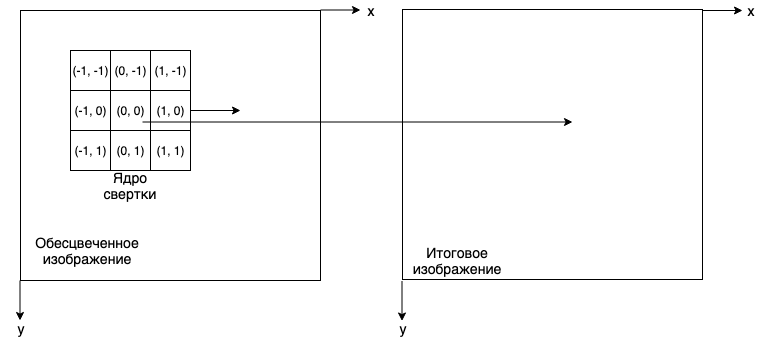
\includegraphics[width=\textwidth,keepaspectratio]{figures/ru/sobel.png}
	\caption{Свертка изображения для получения контура}
	\label{fig:sobel}
\end{figure*}

В итоге значение градиента вычисляется как $G=\sqrt{G_x^2+G_y^2}$, а его направление как $\theta=\arctan(\frac{G_x}{G_y})$.

Результат показывает скорость изменения яркости изображения в конкретной точке, т.е. вероятность ее нахождения на границе изображения.

\subsection{Оператор Прюитт}

Данный метод\cite{Prewitt}, как и оператор Собеля, использует свертку обесцвеченного изображения (рисунок \ref{fig:sobel}) ядром размера 3х3. Отличие заключается в способе задачи маски:

\begin{eqnarray}\label{eq:prewitt-matrixs}
G_x = \begin{bmatrix}
-1 & 0 & 1\\
-1 & 0 & 1\\
-1 & 0 & 1\\
\end{bmatrix} \\
G_y = \begin{bmatrix}
-1 & -1 & -1\\
0 & 0 & 0\\
1 & 1 & 1\\
\end{bmatrix}
\end{eqnarray}

Из-за меньшего значения средних элементов итоговое изображение имеет более явный эффект сглаживания.

\subsection{Перекрестный оператор Робертса}

Рассмотрим область 3х3, представленную ну рисунке \ref{fig:roberst}.

\begin{figure*}[!h]
	\centering
	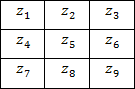
\includegraphics[width=0.2\textwidth,keepaspectratio]{figures/ru/roberts}
	\caption{Окрестность 3х3 внутри изображения}
	\label{fig:roberst}
\end{figure*}

Вычисление первых частных производных, которые обозначают перепад яркости, в точке $z_5$ можно провести следующим образом:

\begin{eqnarray}\label{eq:roberts-eq}
G_x = (z_9 - z_5) \\
G_y = (z_8 - z_6)
\end{eqnarray}

Для вычисления данных производных в каждой точке изображения в данном методе\cite{Roberts} применяется свертка изображения двумя ядрами размера 2х2:

\begin{eqnarray}\label{eq:roberts-matrixs}
\begin{bmatrix}
1 & 0\\
0 & -1
\end{bmatrix} 
\begin{bmatrix}
0 & 1\\
-1 & 0
\end{bmatrix}
\end{eqnarray}

В результате получается изображение пространственного градиента исходного изображения, где точки с наибольшим значением соответствуют границе.

Проблемой данного метода является отсутствие четко выраженного центрального элемента у ядра свертки. Но в следствии этого недостатка алгоритм так же имеет высокую скорость обработки изображения.

\subsection{Оператор Кэнни}

Данный фильтр\cite{Canny} был разработан с учетом удовлетворения следующих свойств:
\begin{itemize}
	\item хорошее обнаружение (Кэнни трактовал это свойство как повышение отношения сигнал/шум);
	\item хорошая локализация (правильное определение положения границы);
	\item единственный отклик на одну границу.
\end{itemize}

Алгоритм состоит из пяти последовательных шагов. Рассмотрим каждый из них подробнее с наглядной визуализацией обработки. Для этого применим данный оператор шаг за шагом к изображению \ref{fig:canny_orig}.

\begin{figure*}[!h]
	\centering
	
\includegraphics[width=0.2\textwidth,keepaspectratio]{figures/ru/bmstu_gray}
	\caption{Исходное изображение для обработки оператором Кэнни}
	\label{fig:canny_orig}
\end{figure*}

\begin{enumerate}
	\item Размытие изображения для удаления лишнего шума. Для этого можно применить фильтр Гаусса\cite{shapiro:2001}.
	Функция, используемая этим фильтром, для двумерного случая задается формулой  \ref{eq:gauss}.
	\begin{eqnarray}\label{eq:gauss}
	Gaus(x, y, \sigma) = \frac{1}{2 \pi \sigma^2}*e^{\frac{-(x^2+y^2)}{2\sigma^2}}
	\end{eqnarray}
	
	Результат применения фильтра Гаусса к изображению \ref{fig:canny_orig} представлен на рисунке \ref{fig:canny_smoothed}
	
	\begin{figure*}[!h]
		\centering
		
\includegraphics[width=0.2\textwidth,keepaspectratio]{figures/ru/bmstu_smoothed}
		\caption{Результат применения фильтра Гаусса}
		\label{fig:canny_smoothed}
	\end{figure*}
	\item Поиск градиентов, для определения границ с максимальным значением градиента.
	На данном этапе можно использовать оператор Собеля \cite{Sobel}, работа которого была описана выше.
	
	Результат поиска градиентов в размытом изображении представлен на рисунке \ref{fig:canny_gradient}.
	
	\begin{figure*}[!h]
		\centering
		
\includegraphics[width=0.2\textwidth,keepaspectratio]{figures/ru/bmstu_gradient}
		\caption{Результат поиска градиентов}
		\label{fig:canny_gradient}
	\end{figure*}

	\item Подавление не-максимумов, т.е. исключение из границ не локальных максимумов.
	
	На данном шаге происходит проверка, является ли конкретный пиксель локальным максимумом вдоль направления градиента. Таким образом исключаются ложные границы.
	
	\begin{figure*}[!h]
		\centering
		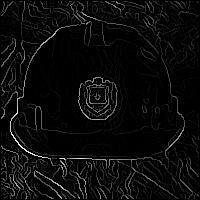
\includegraphics[width=0.2\textwidth,keepaspectratio]{figures/ru/bmstu_non_max}
		\caption{Изображение после подавления не-максимумов}
		\label{fig:canny_non_max}
	\end{figure*}

	\item Определение потенциальных границ с помощью двойной пороговой фильтрации.
	
	Фильтр использует два порога фильтрации:
	\begin{itemize}
		\item Все пиксели со значением больше верхней границы принимают максимальное значение (достоверная граница).
		\item Все пиксели со значением меньше нижней границы подавляются.
		\item Все пиксели со значением в диапазоне границ принимают фиксированное среднее значение. Их уточнение происходит на следующем этапе.
	\end{itemize}

	Пример фильтрации с порогами 0,01 и 0,07 представлен на рисунке \ref{fig:canny_threshold}.
	
	\begin{figure*}[!h]
		\centering
		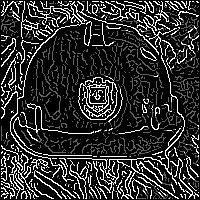
\includegraphics[width=0.2\textwidth,keepaspectratio]{figures/ru/bmstu_threshold}
		\caption{Результат двойной пороговой фильтрации}
		\label{fig:canny_threshold}
	\end{figure*}

	\item Трассировка области неоднозначности
	
	На данном этапе происходит разделение пикселей, получивших промежуточное значение на предыдущем шаге, на границы и фон (увеличение значения и подавление). Пиксель добавляется к границе, если он соприкасается с ней по одному из 8-ми направлений.
	
	Результат работы оператора Кэнни представлен на рисунке \ref{fig:canny_final}.
	
	\begin{figure*}[!h]
		\centering
		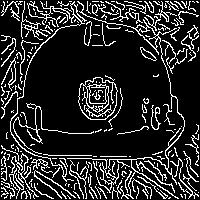
\includegraphics[width=0.2\textwidth,keepaspectratio]{figures/ru/bmstu_final}
		\caption{Результат работы оператора Кэнни}
		\label{fig:canny_final}
	\end{figure*}
\end{enumerate}


Стоит обратить внимание, что описанные выше методы принимают на вход изображение в серых тонах. То есть нулевым шагом данных методов можно указать преобразование изображения из цветного в черно-белое.


\section{Выделение силуэта кисти руки}
\label{sec:Threholding}

Помимо классических методов определения границ можно использовать сегментацию по цвету кожи \cite{Phung}. Данный метод преобразует RGB изображение в бинарное с помощью фильтрации пикселей по цвету, близкому к цвету кожи. Для улучшения работы алгоритма перед фильтрацией изображение переводят в цветовое пространство YCrCb, в котором различные цвета кожи  расположены близко друг к другу \cite{Siddharth}.

Пример фильтрации изображения: 

\begin{minipage}{0.75\textwidth}
	\begin{algorithm}[H]
		\lstinputlisting[language=Python]{src/color_filter.py}
		\caption{Фильтрация изображения по цвету кожи}
		\label{imp:color-filter}
	\end{algorithm}
\end{minipage}

В большинстве случаев после бинаризации на изображении присутствуют шумы и артефакты, вызванные тем, что на фоновой части изображения находились пиксели, попадающие в ограничения фильтра. Для их устранения можно использовать морфологические операции "расширение" и "сужение" \cite{DIP}:

\begin{minipage}{0.75\textwidth}
	\begin{algorithm}[H]
		\lstinputlisting[language=Python]{src/color_noise.py}
		\caption{Применение к изображению операций расширение и сужение}
		\label{imp:color-noise}
	\end{algorithm}
\end{minipage}

\section{Построение скелета кисти руки}
\label{sec:Skeleton}

\section{Методология}
\label{sec:Method}

Для сравнительного анализа описанных выше методов они были реализованы на языке Python 3 с использованием следующих библиотек:

\begin{itemize}
	\item Python Imaging Library
	\item scipy
	\item numpy
	\item OpenCV
\end{itemize} 

Каждый алгоритмом был обработан одинаковый набор данных, состоящий из растровых изображений кистей рук тестовая выборка составлялась из нескольких наборов данных, различающиеся разными форматами изображений, их размерами и людьми, чьи руки использовались для получения изображений кистей. Все данные находятся в открытом доступе:

\begin{itemize}
	\item ASL Alphabet. Image data set for alphabets in the American Sign Language\footnote{https://www.kaggle.com/grassknoted/asl-alphabet}. Данный датасет состоит из 87000 изображений американского дактиля в обучающей выборке и 29 проверочных изображений. Каждое изображение цветное, сохранено в формате JPG, имеет размерность 200x200 пикселей. Для проверки работы алгоритмов были использованы проверочные изображения.
	
	\item Hand Gesture of the Colombian sign language. Hand gestures, recognizing the numbers from 0 to 5 and the vowels\footnote{https://www.kaggle.com/evernext10/hand-gesture-of-the-colombian-sign-language}. Данный датасет состоит из фотографий жестов, изображающий гласные буквы колумбийского языка и цифры от 0 до 5. Приведены снимки как мужских, так и женских рук. Каждый жест имеет 3 разных фото с разных ракурсов. Каждое изображение цветное, сохранено в формате JPG, имеет размерность 4608 x 2592 пикселей. Для проверки работы алгоритмов были отобраны случайные изображения, по одному на каждый жест.
	
	\item ASL Fingerspelling Images (RGB \& Depth) \footnote{https://www.kaggle.com/mrgeislinger/asl-rgb-depth-fingerspelling-spelling-it-out}. Данная выборка состоит из изображений американского дактиля. В выборке участвуют 5 разных людей, у каждого человека на каждый символ приходится более 1000 изображений. Все изображения цветные, формата PNG, имеют различную размерность. Для проверки работы алгоритмов были отобраны случайным образом по одному изображению для каждой буквы, то есть в итоговой выборке участвовали снимки разных людей под разными ракурсами.
	
	\item sign language between 0 9\footnote{https://www.kaggle.com/beyzance96/sign-language-between-0-9}. Данная выборка состоит из изображений жестов, обозначающих цифры от 0 до 10. Все изображения цветные, формата JPG, размерности 300x300. Данные разделены на обучающие, где на каждую цифру приходится более 100 различных изображений, и проверочные, где на каждую цифру представлено одно изображение. Для проверки работы алгоритмов были выбраны все изображения из проверочной выборки. 
	
\end{itemize}

 Были проведены замеры времени обработки каждого изображения для получения статистики по минимальному, максимальному и среднему времени работы алгоритма.

%\section{Data}
\label{sec:Data}

This section describes the data used in this work, justified their choice, as well as specify their sources. A common practice is to analyze the descriptive statistics, allows to make some assumptions even before the results of the study.

\section{Результаты}
\label{sec:Results}

В данном разделе приводятся основные полученные в работе результаты, а также выполняется их детальный анализ.

\subsection{Название параграфа}
\label{sec:}

\begin{table*}[!h]
\caption{Пример простой таблицы, содержащей описательную статистику.}
\label{tab:tab_descr_1}
\setlength{\arrayrulewidth}{1.05 pt}
\renewcommand{\arraystretch}{1.1}
\begin{tabular*}{1.0\textwidth}{@{\extracolsep{\fill}}lrr}
\hline
Параметр & Название колонки & Название колонки \\
\hline
Среднее, $\mu$ & 0.79 & 0.98 \\
\hline
\end{tabular*}
\begin{spacing}{0.5}
{\scriptsize Пояснения: Здесь даются пояснения к таблице.}
\end{spacing}
\end{table*}

\subsection{Название параграфа}
\label{sec:}

\begin{table*}[!h]
\caption{Пример более сложной таблицы, содержащей оценки параметров модели.}
\label{tab:}
\setlength{\arrayrulewidth}{1.05 pt}
\renewcommand{\arraystretch}{1.1}
\begin{tabular*}{1.0\textwidth}{@{\extracolsep{\fill}}lrrr}
\hline
Параметр & \textit{Название колонки} & \textit{Название колонки} & \textit{Название колонки} \\
\hline

\multicolumn{4}{l}{\textit{Группа 1}} \\
$\mu$ & 0.30\textsuperscript{***} {\footnotesize (0.01)} & 0.30\textsuperscript{***} {\footnotesize (0.01)} & 0.30\textsuperscript{***} {\footnotesize (0.01)} \\
$\phi$ & 0.30\textsuperscript{***} {\footnotesize (0.01)} & 0.30\textsuperscript{***} {\footnotesize (0.01)} & 0.30\textsuperscript{***} {\footnotesize (0.01)} \\

\multicolumn{4}{l}{\textit{Группа 2}} \\
$\mu$ & 0.40\textsuperscript{*} {\footnotesize (0.17)} & 0.40\textsuperscript{*} {\footnotesize (0.17)} & 0.40\textsuperscript{*} {\footnotesize (0.17)} \\
$\phi$ & 0.40\textsuperscript{*} {\footnotesize (0.17)} & 0.40\textsuperscript{*} {\footnotesize (0.17)} & 0.40\textsuperscript{*} {\footnotesize (0.17)} \\

\hline
\end{tabular*}
\begin{spacing}{0.5}
{\scriptsize Пояснения: В скобках приведены стандартные ошибки параметров. Уровни значимости: *** -- 1\%, ** -- 5\%, * -- 10\%.}
\end{spacing}
\end{table*}

\subsection{Название параграфа}
\label{sec:}

\begin{figure*}[!h]
\centering
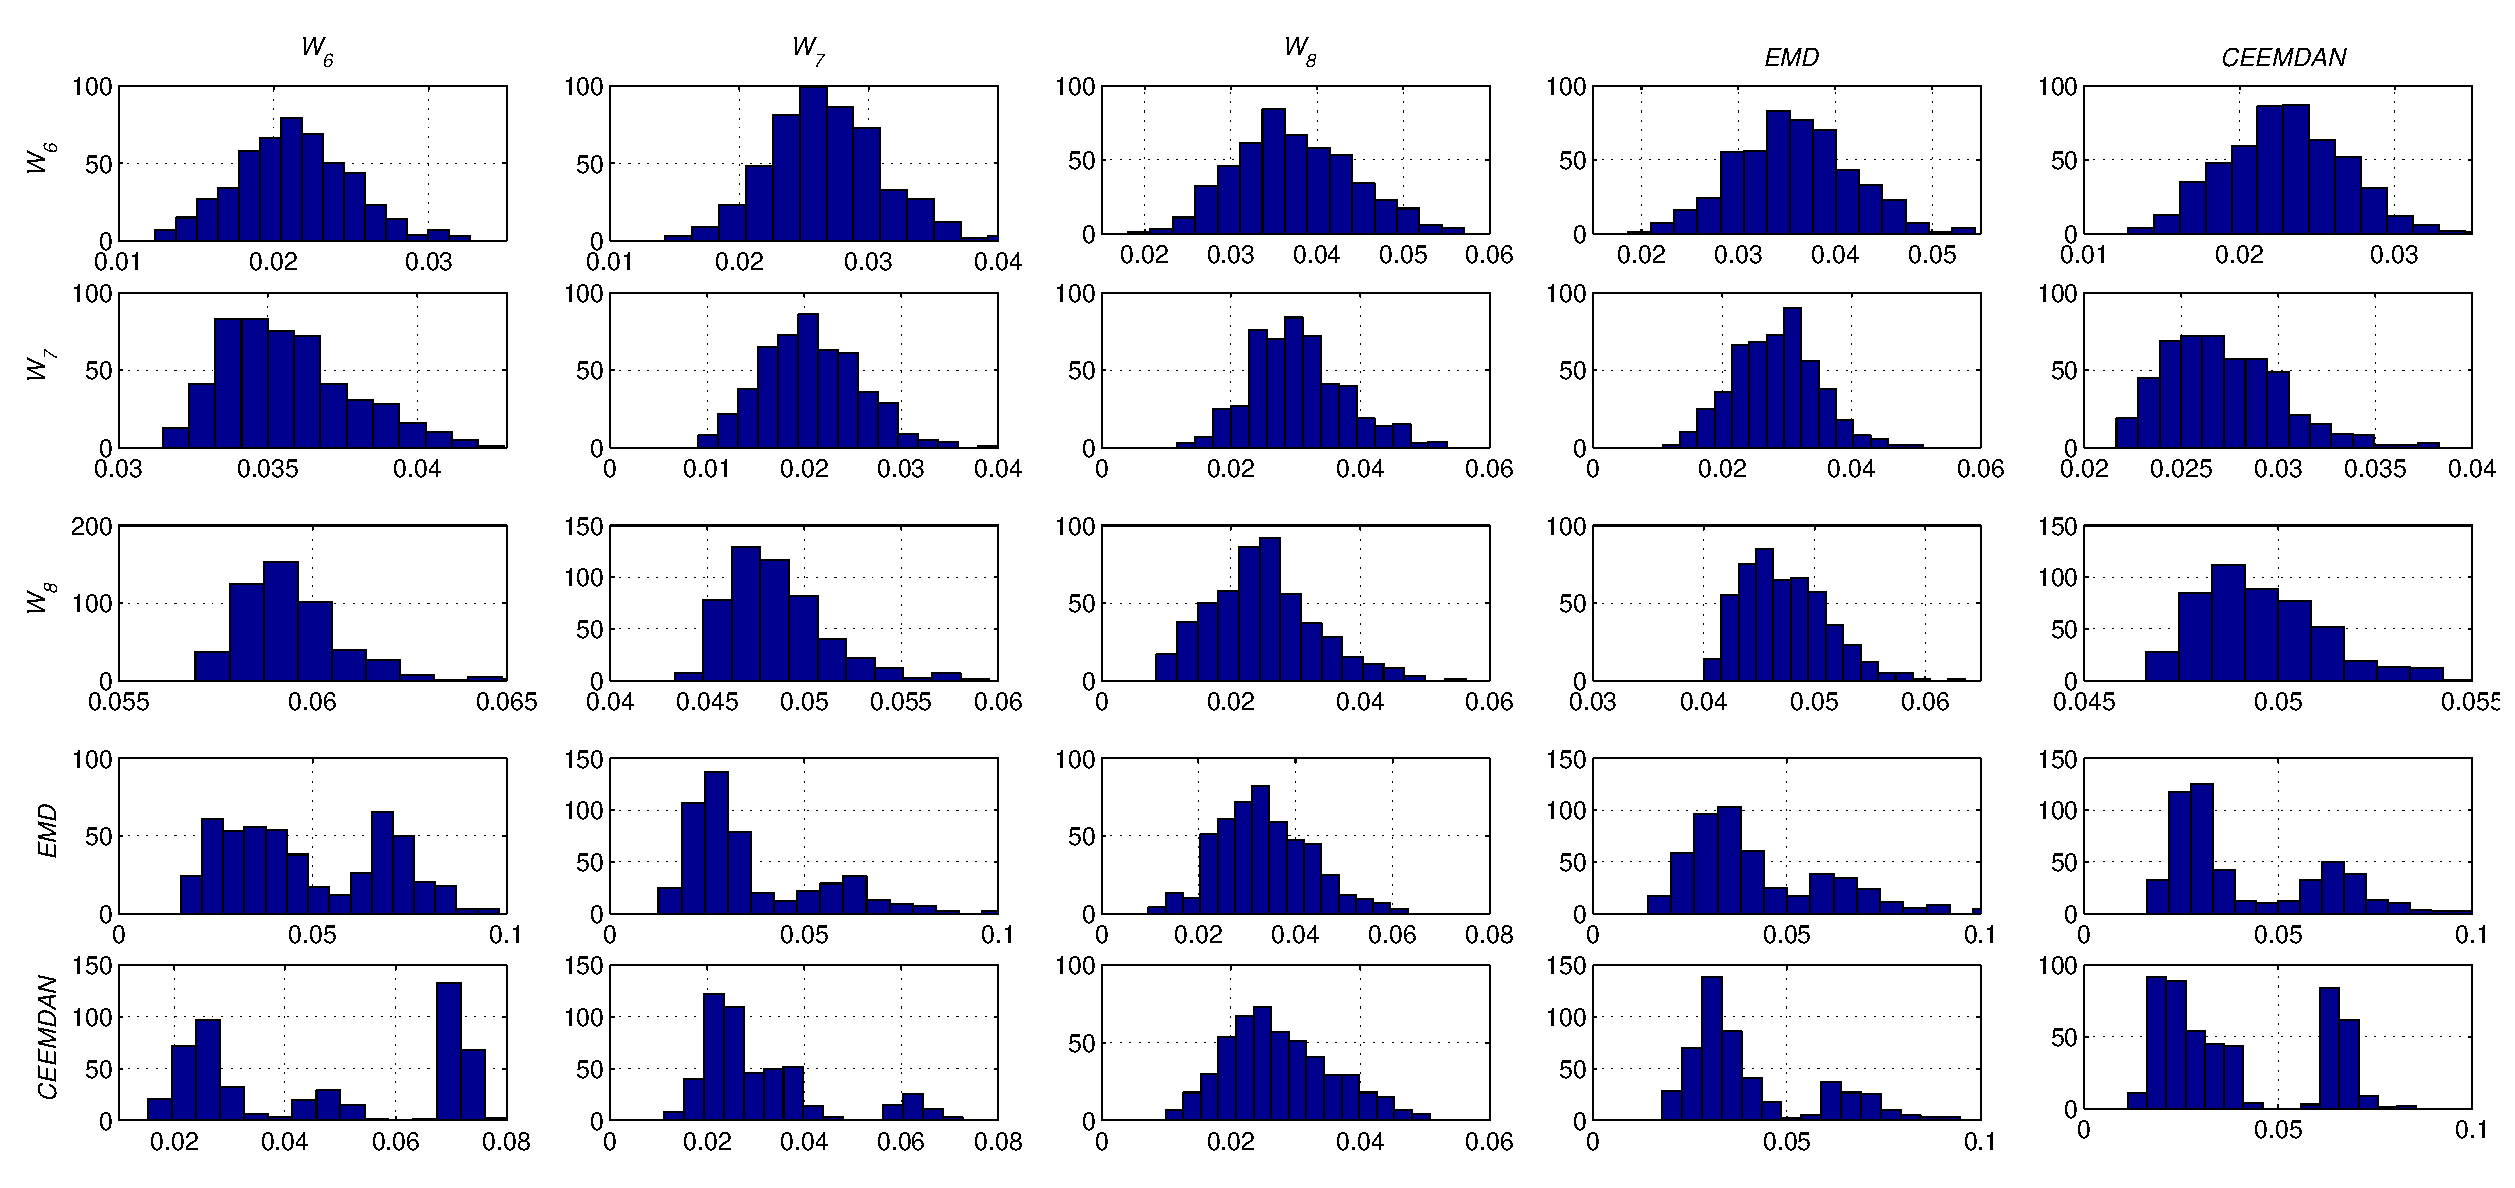
\includegraphics[width=1.0\textwidth,keepaspectratio]{Figure}
\caption{Название рисунка.}
\label{fig:}
\end{figure*}

\section{Conclusion}
\label{sec:Conclusion}

This section summarizes the results and draws the main conclusions of the study.

%\section{Благодарности}
\label{sec:Acknowledgement}

Раздел содержит благодарности людям или организациям, которые оказали существенную помощь различного характера при написании работы.

В качестве базового, можно использовать следующий шаблон:

Авторы выражают благодарность \{ФИО\} за ценные комментарии по содержанию работы. Ответственность за все ошибки и неточности, допущенные авторами, лежит исключительно на них самих.
\section*{Список литературы}
\bibliographystyle{unsrt}
\bibliography{biblio}

\appendix
\section{Название приложения}
\label{sec:Appendix_}

\begin{figure*}[!h]
	\centering
	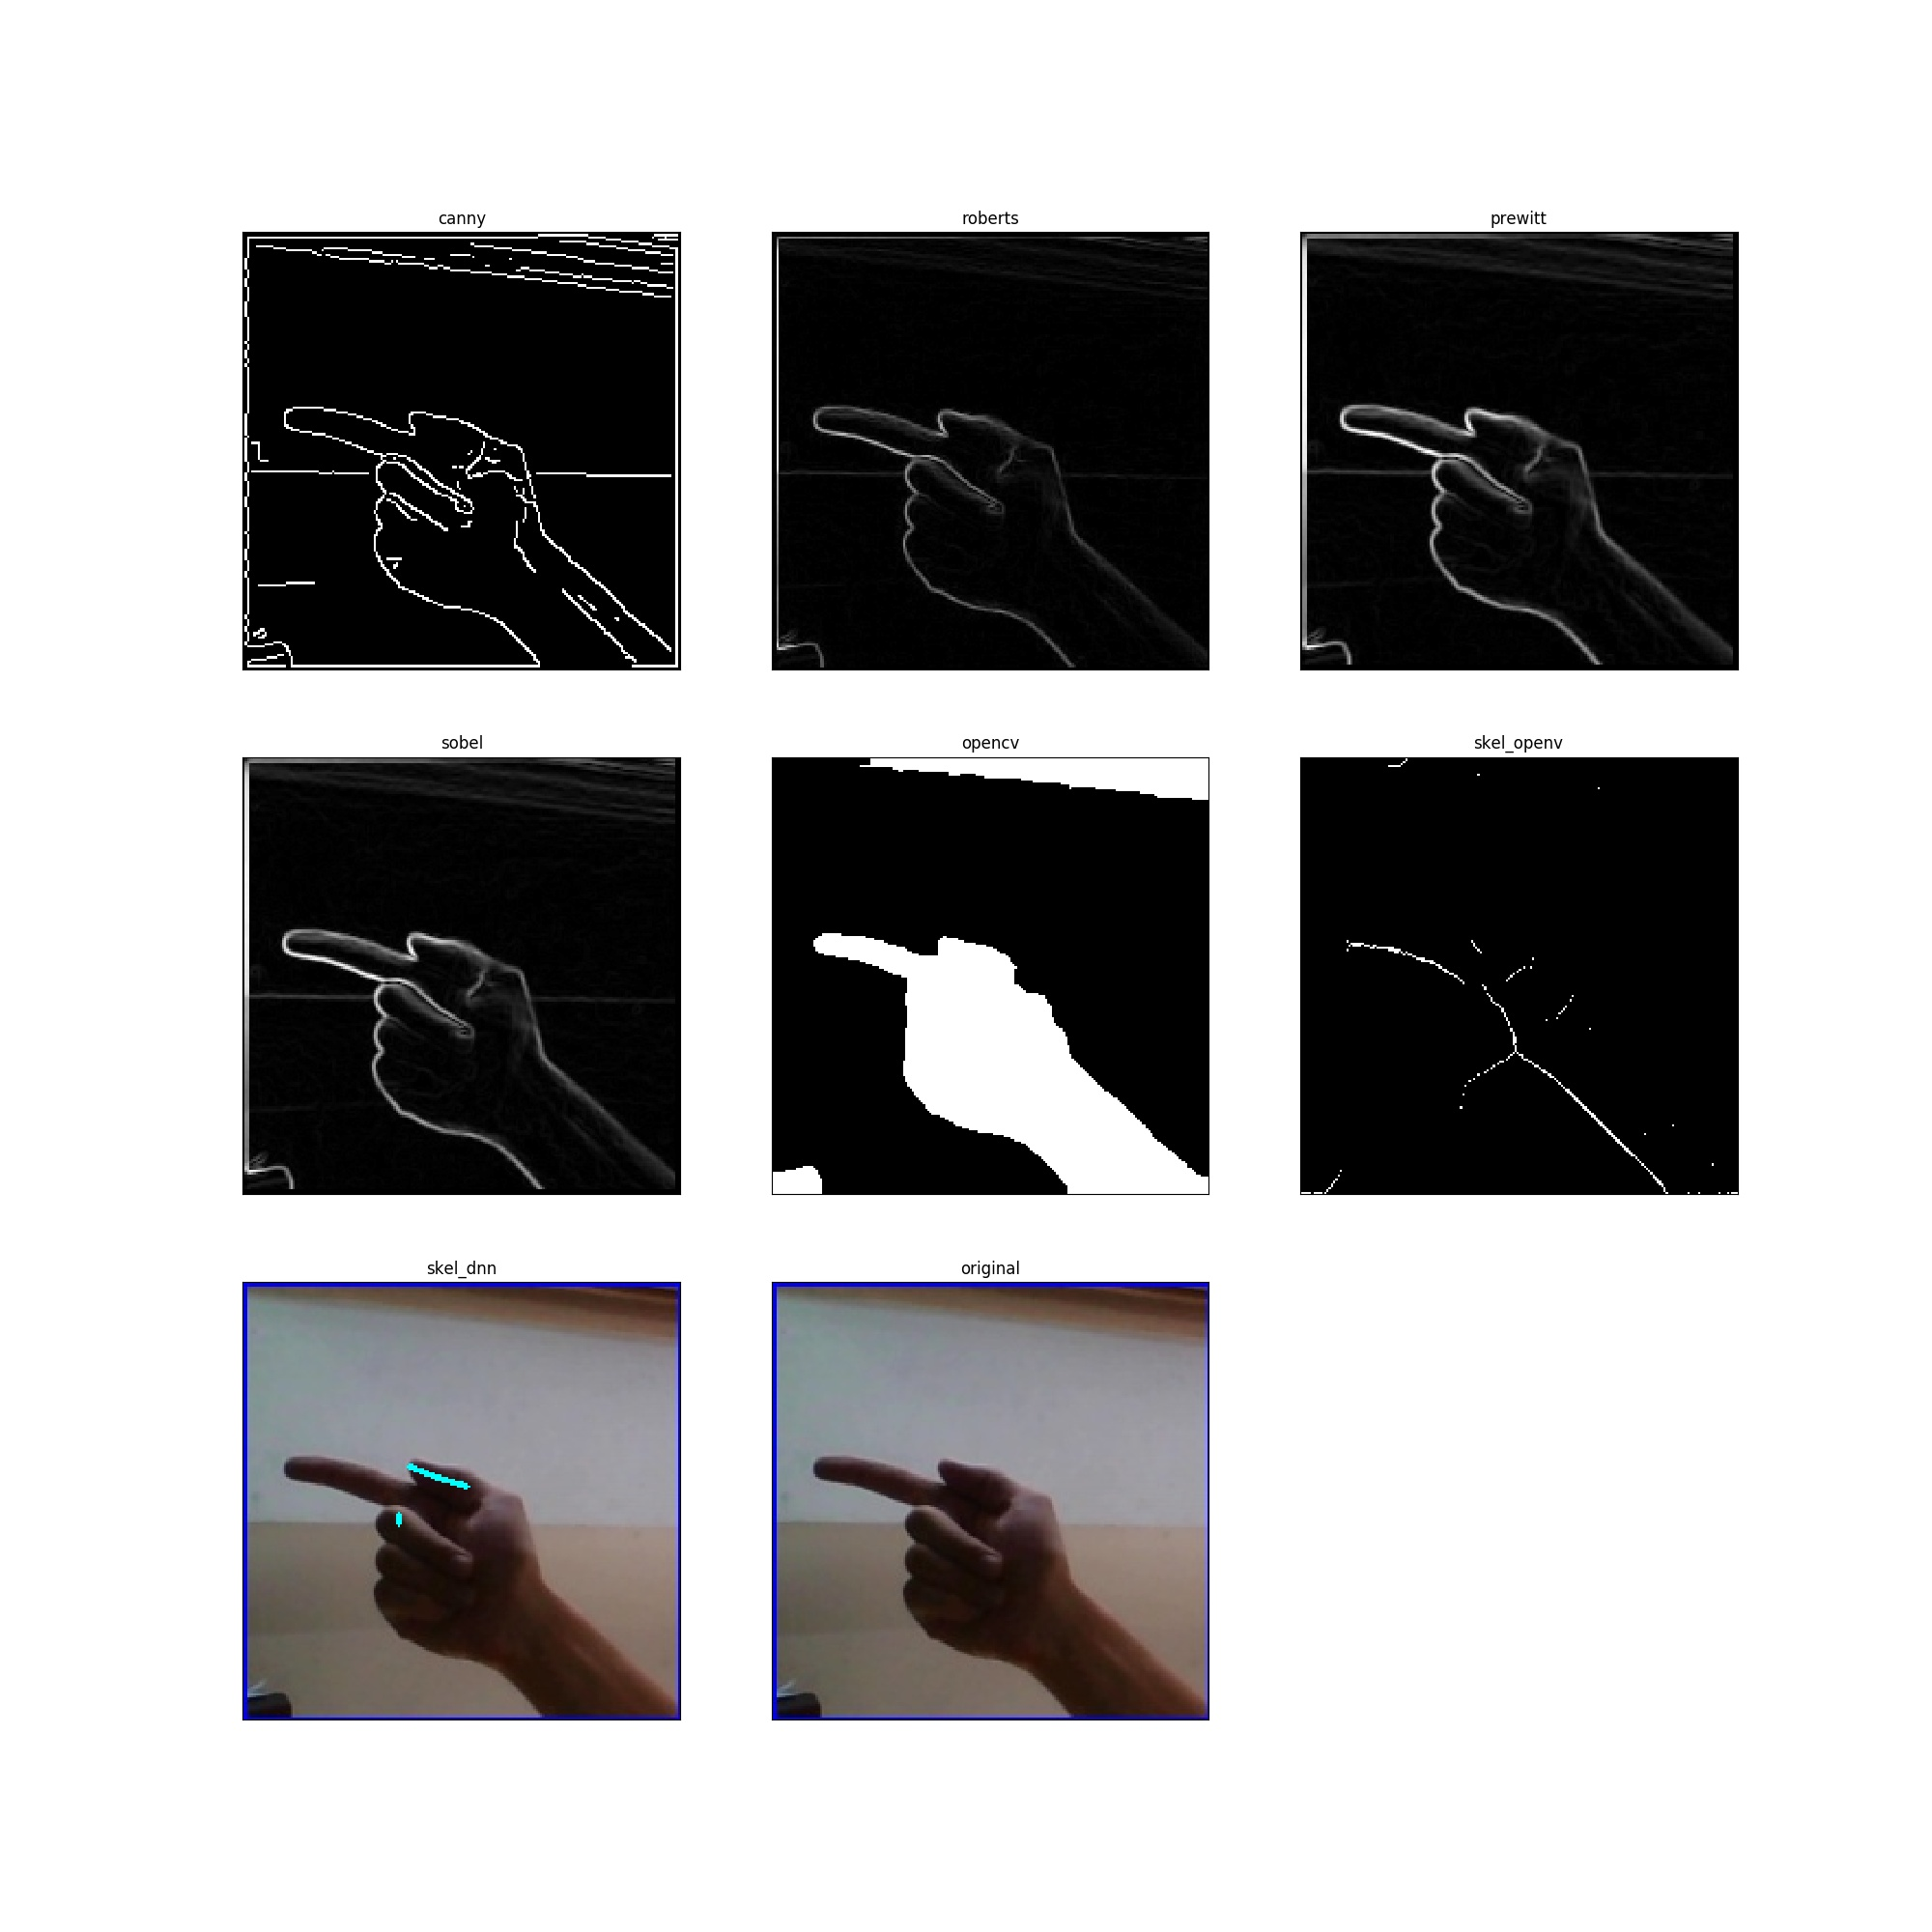
\includegraphics[width=\textwidth,keepaspectratio]{figures/ru/asl.jpg}
	\caption{Результат работы алгоритмов (в секундах) на наборе данных ASL Alphabet}
	\label{fig:asl}
\end{figure*}

\begin{figure*}[!h]
	\centering
	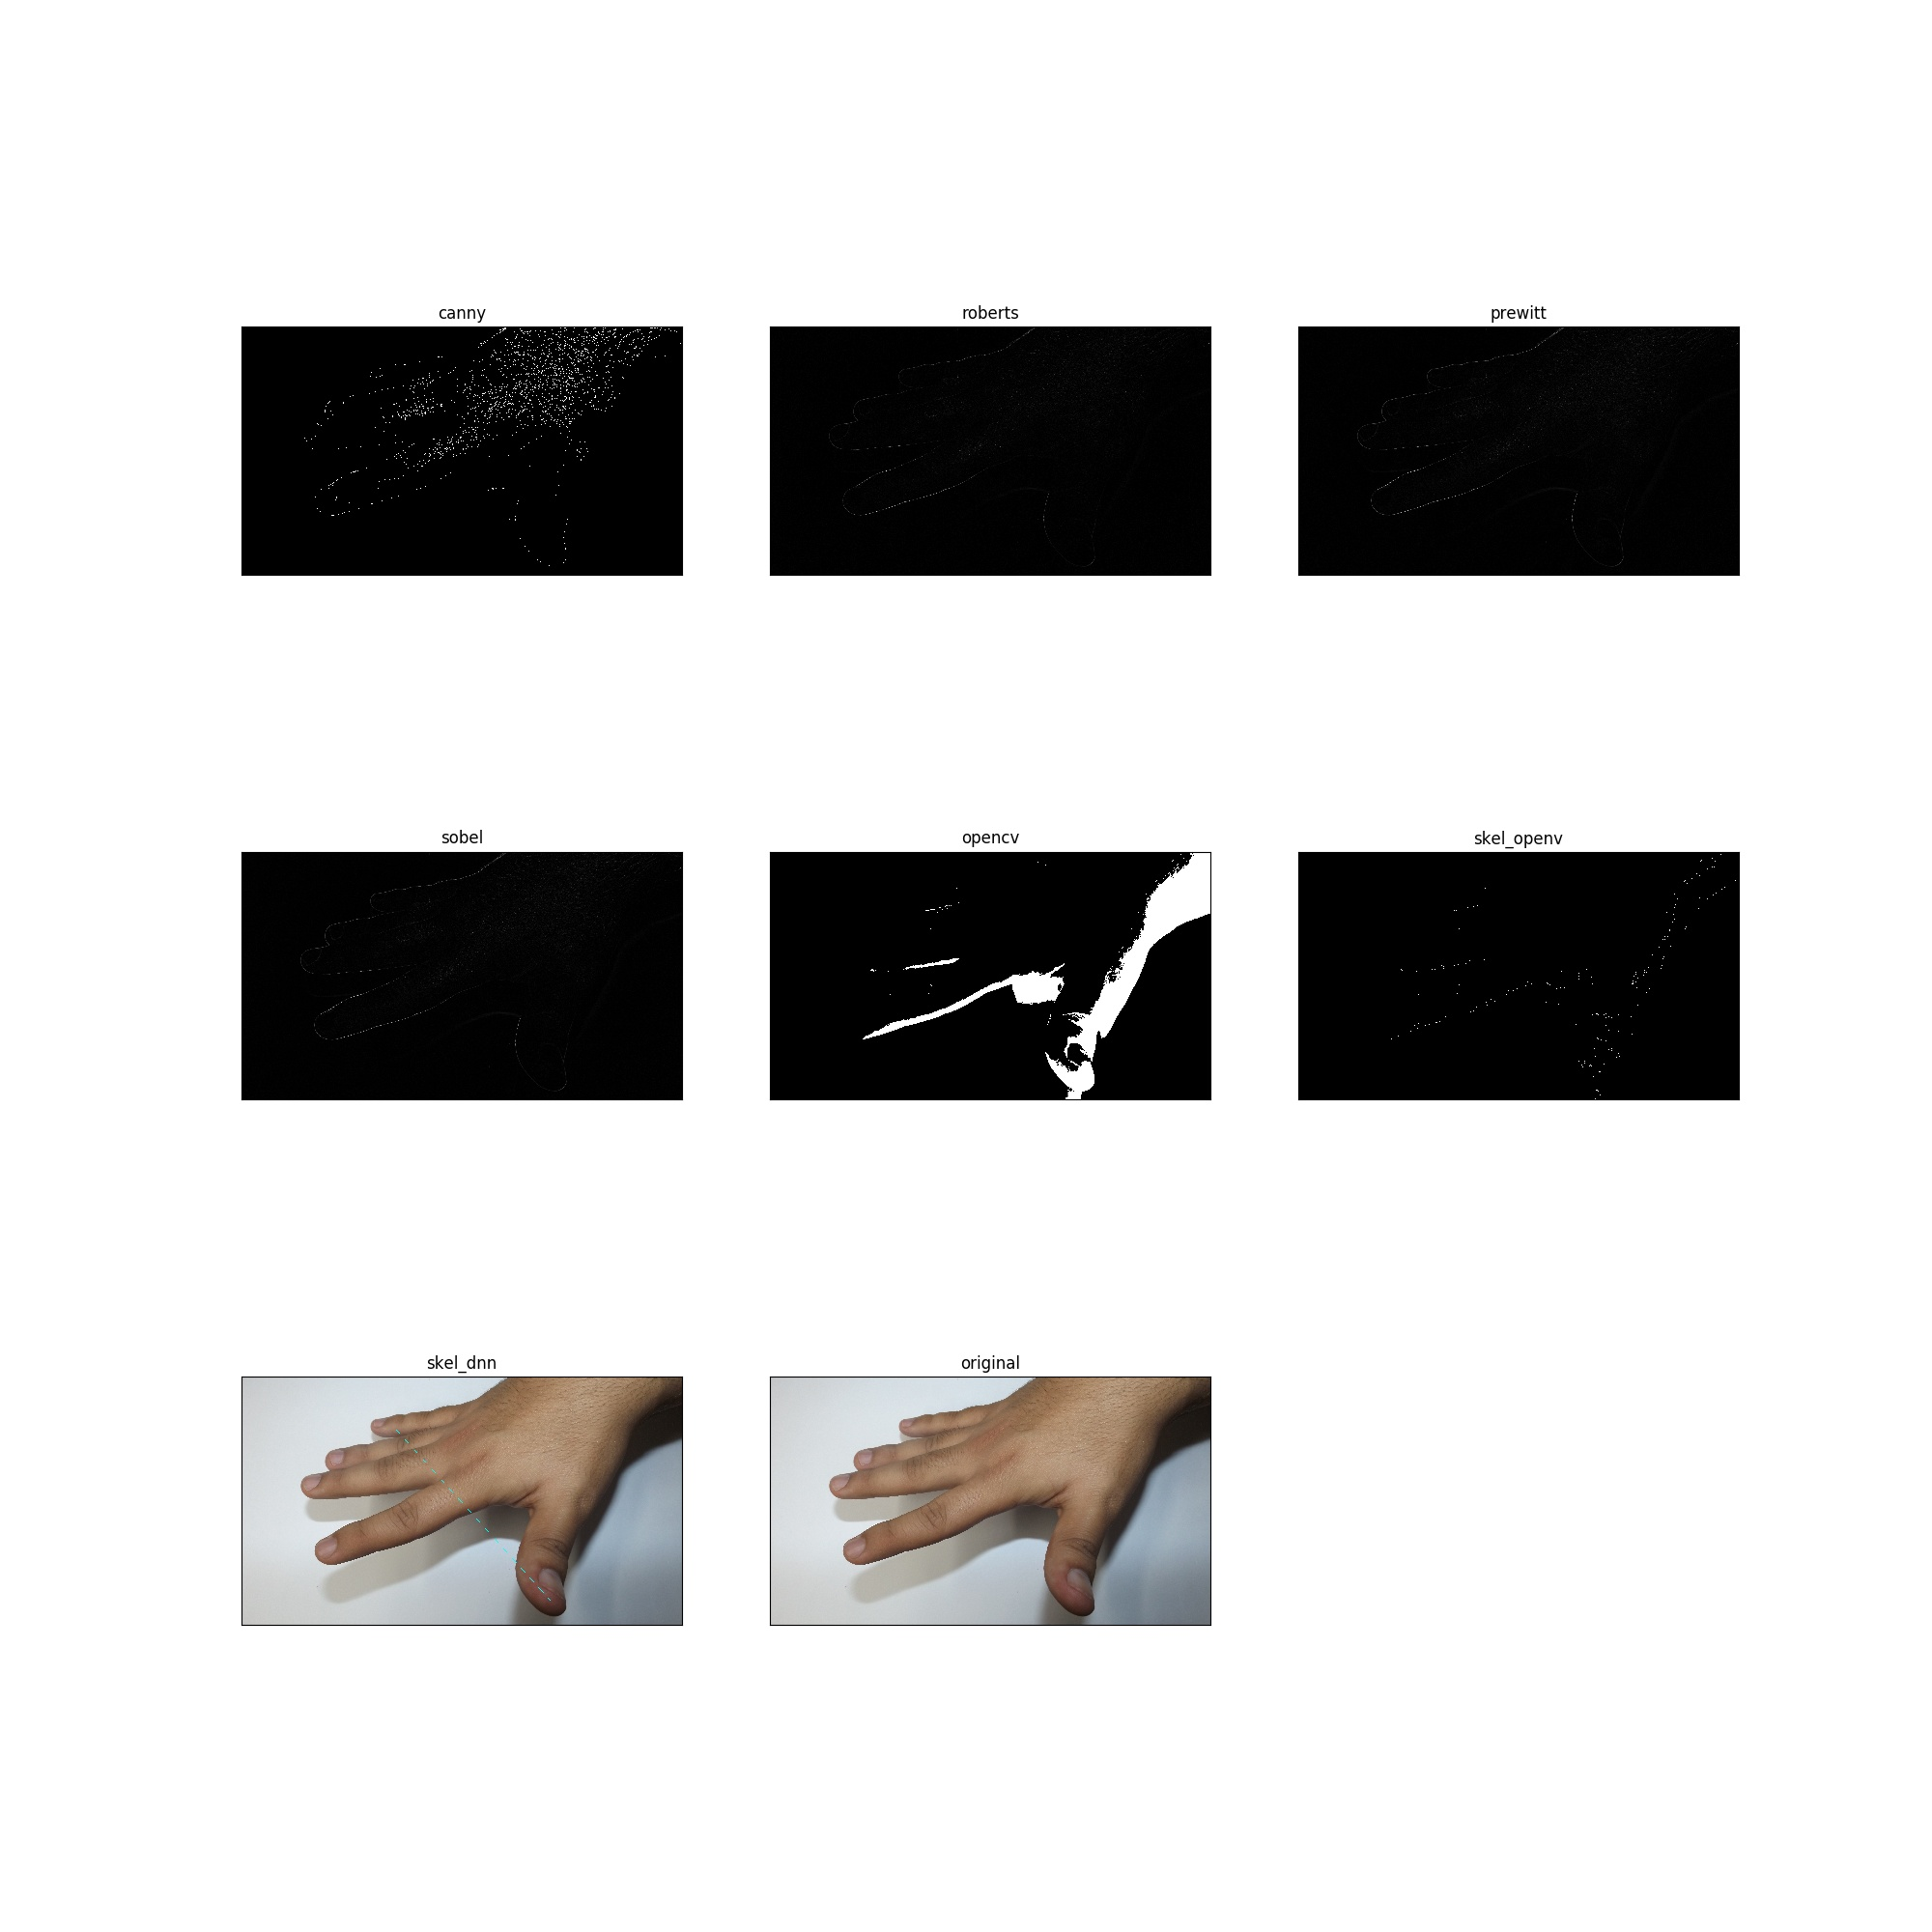
\includegraphics[width=\textwidth,keepaspectratio]{figures/ru/coombian.jpg}
	\caption{Результат работы алгоритмов (в секундах) на наборе данных Hand Gesture of the Colombian sign language}
	\label{fig:colombian}
\end{figure*}

\begin{figure*}[!h]
	\centering
	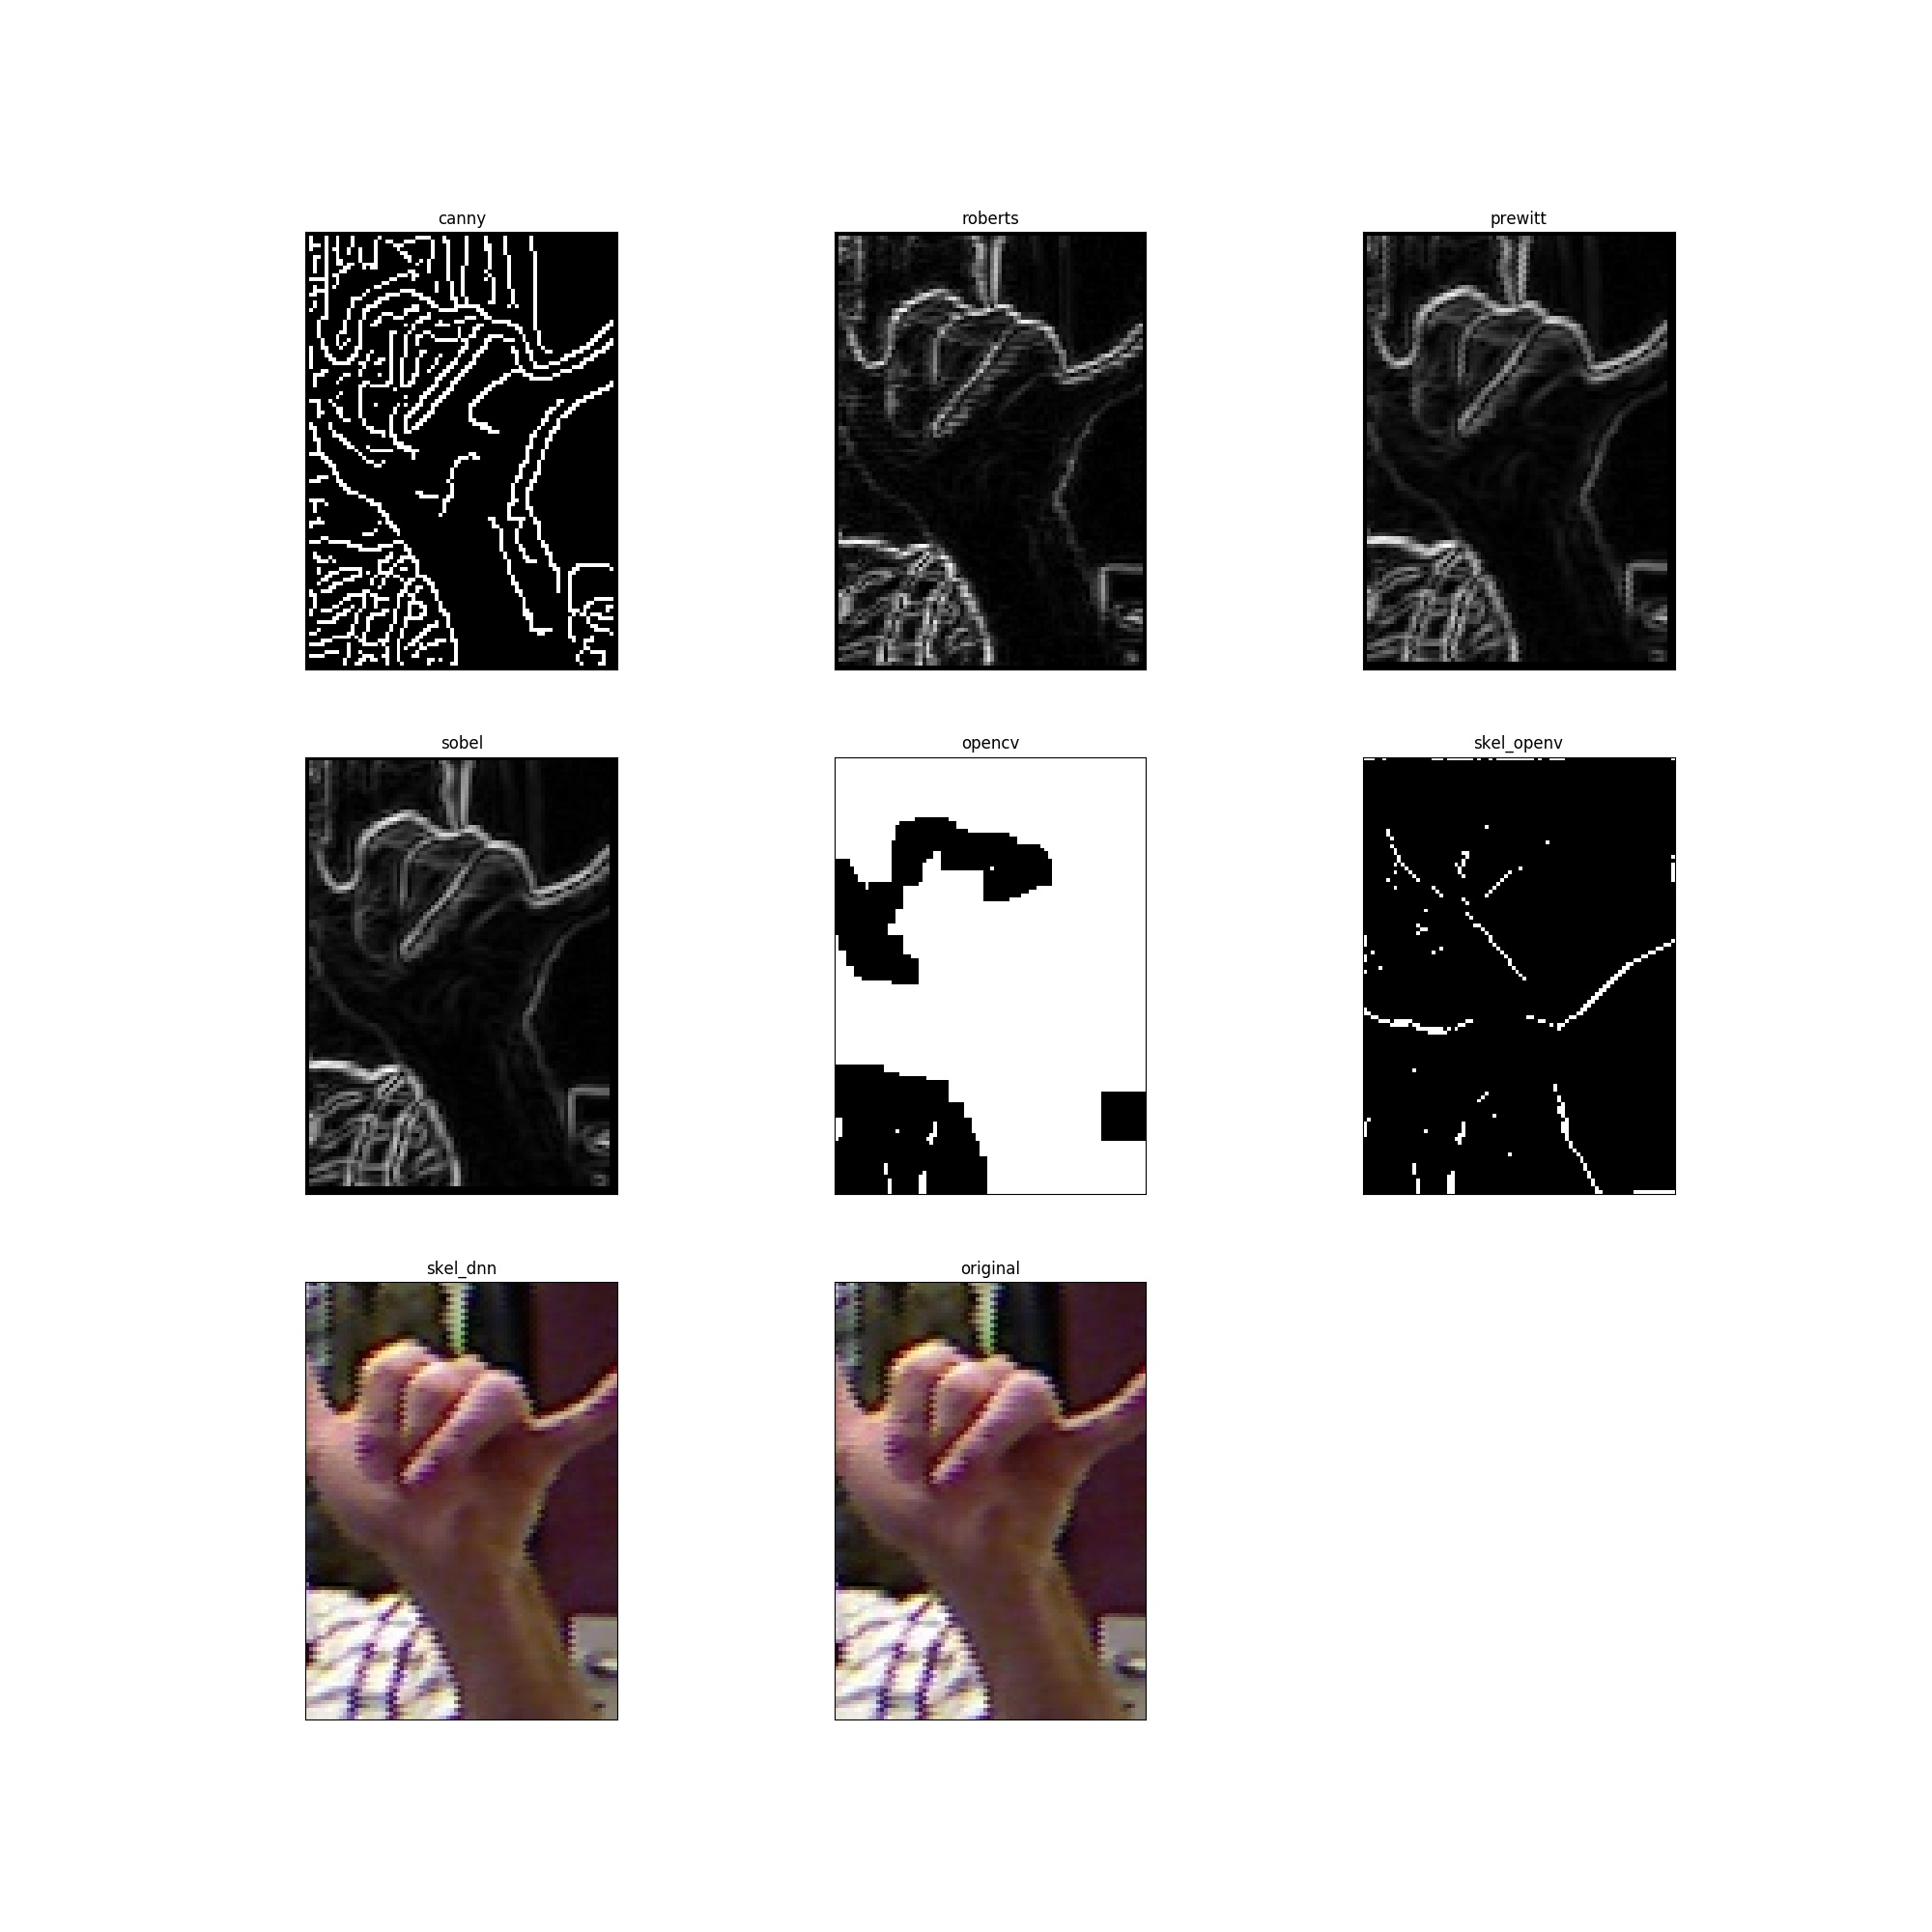
\includegraphics[width=\textwidth,keepaspectratio]{figures/ru/asl2.jpg}
	\caption{Результат работы алгоритмов (в секундах) на наборе данных ASL Fingerspelling Images}
	\label{fig:asl2}
\end{figure*}

\begin{figure*}[!h]
	\centering
	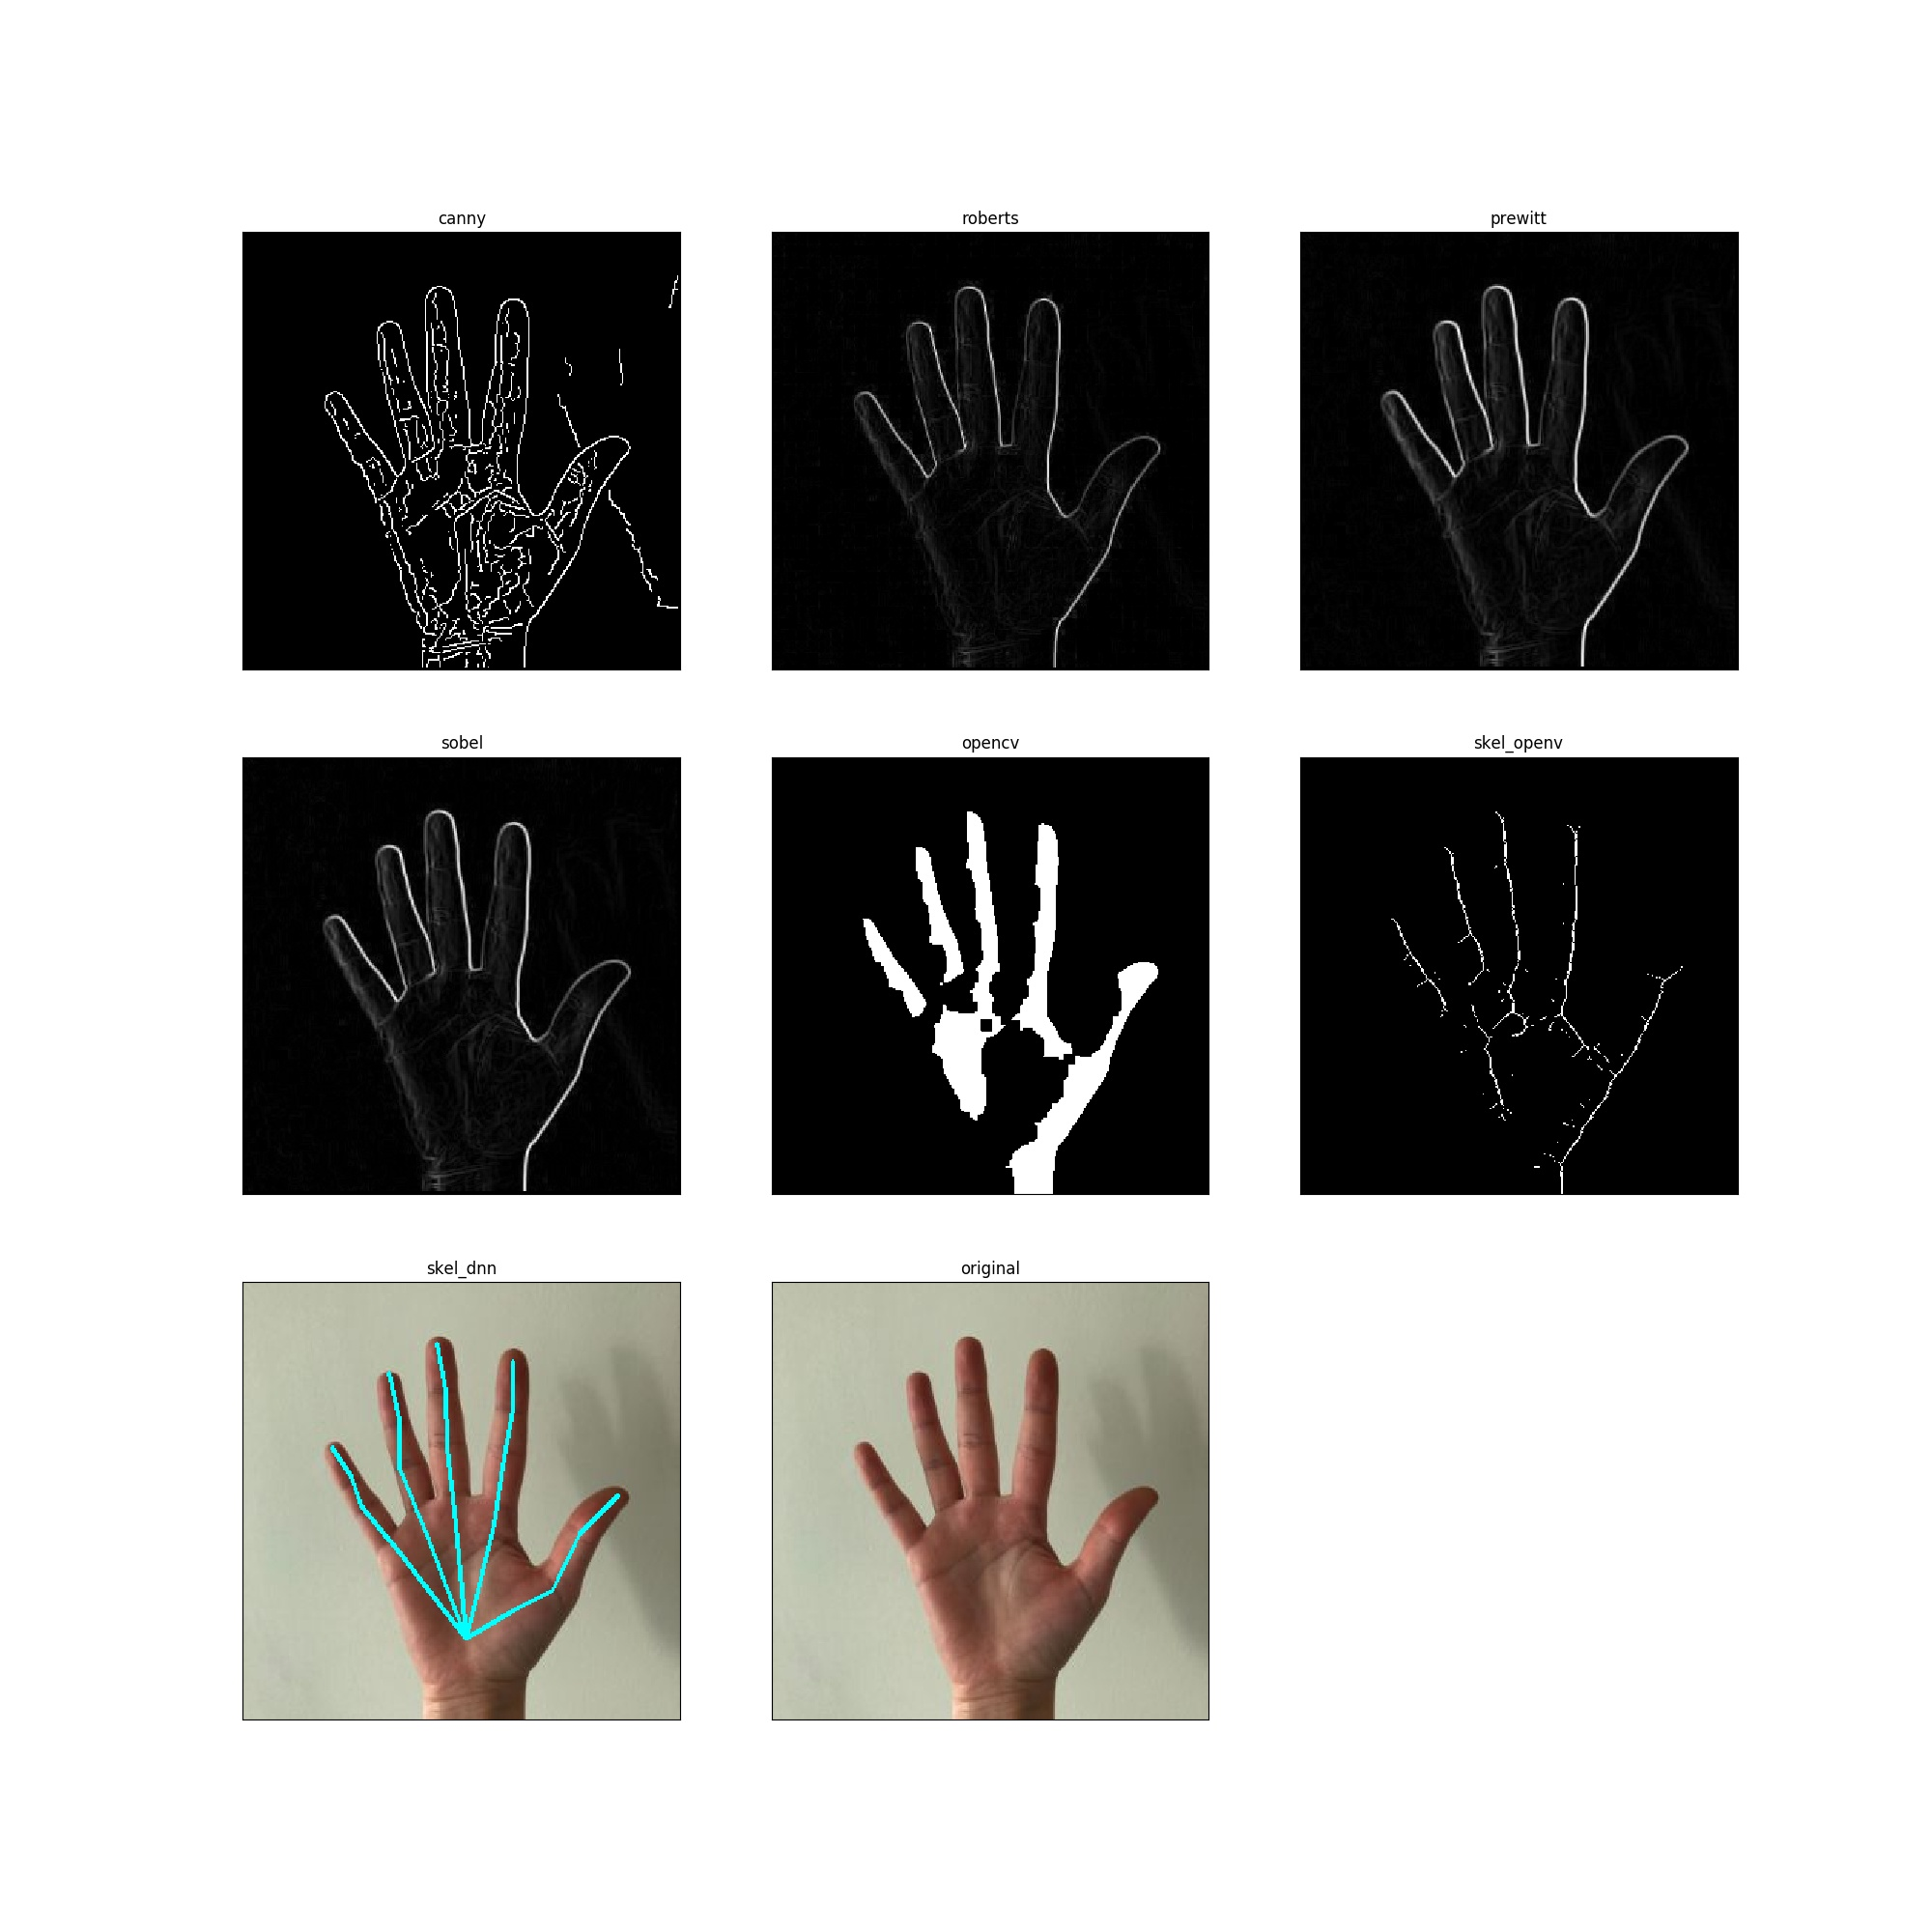
\includegraphics[width=\textwidth,keepaspectratio]{figures/ru/datamix.jpg}
	\caption{Результат работы алгоритмов (в секундах) на наборе данных sign language between 0 9}
	\label{fig:datamix}
\end{figure*}

\begin{table*}[!h]
\caption{Время работы алгоритмов (в секундах) на наборе данных ASL Alphabet}
\label{tab:asl-alphaber}
\setlength{\arrayrulewidth}{1.05 pt}
\renewcommand{\arraystretch}{1.1}
\begin{tabular*}{1.0\textwidth}{@{\extracolsep{\fill}}|c|c|c|c|}
	\hline
	Название алгоритма & Минимальное время & Максимальное время & Среднее время \\
	\hline
	Оператор Кэнни & 0.1783 & 0.4642 & 0.2553 \\
	Оператор Робертса & 0.0687 & 0.1252 & 0.0852 \\
	Оператор Прюитт & 0.1175 & 0.2211 & 0.1424  \\
	Оператор Собеля & 0.1177 & 0.3112 & 0.1527 \\
	Выделение силуэта & 0.0668 & 0.2101 & 0.0901 \\
	\specialcell{Морфологическое \\ построение скелета} & 0.2084 & 1.2112 & 0.3068 \\
	\specialcell{Построение скелета \\ по ключевым точкам} & 1.408 & 3.4571 & 2.042 \\
	\hline
\end{tabular*}
\end{table*}

\begin{table*}[!h]
\caption{Время работы алгоритмов (в секундах) на наборе данных Hand Gesture of the Colombian sign language}
\label{tab:colombian-alphaber}
\setlength{\arrayrulewidth}{1.05 pt}
\renewcommand{\arraystretch}{1.1}
\begin{tabular*}{1.0\textwidth}{@{\extracolsep{\fill}}|c|c|c|c|}
	\hline
	Название алгоритма & Минимальное время & Максимальное время & Среднее время \\
	\hline
	Оператор Кэнни & 53.5126 & 72.6076 & 62.971 \\
	Оператор Робертса & 22.2837 & 54.2706 & 25.8842 \\
	Оператор Прюитт & 38.7491 & 99.2961 & 46.5944 \\
	Оператор Собеля & 38.8739 & 104.1867 & 46.9016 \\
	Выделение силуэта & 22.3001 & 32.8930 & 23.5992 \\
	\specialcell{Морфологическое \\ построение скелета} & 65.3335 & 88.3565 & 69.0014 \\
	\specialcell{Построение скелета \\ по ключевым точкам} & 3.0844 & 4.2156 & 3.2775 \\
	\hline
\end{tabular*}
\end{table*}

\begin{table*}[!h]
\caption{Время работы алгоритмов (в секундах) на наборе данных ASL Fingerspelling Images}
\label{tab:asl2-alphaber}
\setlength{\arrayrulewidth}{1.05 pt}
\renewcommand{\arraystretch}{1.1}
\begin{tabular*}{1.0\textwidth}{@{\extracolsep{\fill}}|c|c|c|c|}
	\hline
	Название алгоритма & Минимальное время & Максимальное время & Среднее время \\
	\hline
	Оператор Кэнни & 0.0193 & 0.0816 & 0.0545 \\
	Оператор Робертса & 0.0111 & 0.0476 & 0.0286 \\
	Оператор Прюитт & 0.0179 & 0.0864 & 0.0495 \\
	Оператор Собеля & 0.0217 & 0.0847 & 0.0469 \\
	Выделение силуэта & 0.0114 & 0.0506 & 0.0277 \\
	\specialcell{Морфологическое \\ построение скелета} & 0.0343 & 0.1852 & 0.0884 \\
	\specialcell{Построение скелета \\ по ключевым точкам} & 0.6251 & 3.3092 & 1.5665 \\
	\hline
\end{tabular*}
\end{table*}

\begin{table*}[!h]
	\caption{Время работы алгоритмов (в секундах) на наборе данных sign language between 0 9}
	\label{tab:datamix-alphaber}
	\setlength{\arrayrulewidth}{1.05 pt}
	\renewcommand{\arraystretch}{1.1}
	\begin{tabular*}{1.0\textwidth}{@{\extracolsep{\fill}}|c|c|c|c|}
		\hline
		Название алгоритма & Минимальное время & Максимальное время & Среднее время \\
		\hline
		Оператор Кэнни & 0.333 & 0.7686 & 0.4708 \\
		Оператор Робертса & 0.1566 & 0.246 & 0.1778 \\
		Оператор Прюитт & 0.271 & 0.3751 & 0.3027 \\
		Оператор Собеля & 0.2718 & 0.655 & 0.3295 \\
		Выделение силуэта & 0.1486 & 0.4709 & 0.2085 \\
		\specialcell{Морфологическое \\ построение скелета} & 0.4471 & 1.637 & 0.6518 \\
		\specialcell{Построение скелета \\ по ключевым точкам} & 1.4346 & 3.2976 & 2.0723 \\
		\hline
	\end{tabular*}
\end{table*}

%% bibliography
\phantomsection
\addcontentsline{toc}{section}{Список литературы}
\end{document}